% -*-latex-*-

%% Defines the cover material, including the title page, copyright page,
%% signature page, abstract, and acknowledgements.

% All of these pages have special geometry; undo tufte-latex's big margin
\newgeometry{left=3.5cm,bottom=0.1cm}

\title{Multiscale analysis of infectious diseases:\\
       Integrating omics and clinical informatics data into patient care}
\fancytitle{
  \def\baselinestretch{1.1}\Huge
  \textcolor{AccentColor}{\smallcapsspacing{\MakeUppercase{Multiscale analysis}}}\\
  \textit{of}\\
  \textcolor{AccentColor}{\smallcapsspacing{\MakeUppercase{infectious diseases}}}\\
  \vspace{1cm}
  \LARGE
  \smallcapsspacing{\MakeLowercase{\scshape Integrating omics and clinical informatics data}}\\
  \def\baselinestretch{0.5}
  \smallcapsspacing{\MakeLowercase{\scshape into patient care}}
}
\author{Theodore Robertson Pak}

\degree{Doctor of Philosophy}
\program{Biomedical Sciences Doctoral Program}
\department{Graduate School of Biomedical Sciences}
\school{Icahn School of Medicine at Mount Sinai}

\degreemonth{April}
\degreeyear{2017}
\thesisdate{April 27, 2017}

\supervisor{Andrew Kasarskis, PhD}
\dean{Marta Filizola, PhD}{Dean of the Graduate School of Biomedical Sciences}

\committeemembers{
  James Iatridis, PhD (chair)\\
  Adolfo García-Sastre, PhD\\
  Joel Dudley, PhD\\
  Jonathan Karr, PhD\\
  Jun Zhu, PhD\\
  Bo Shopsin, MD, PhD (outside reviewer)
}

\signedsignaturepage{figs/thesis-signature-page-signed-fixed.pdf}

% Make the titlepage based on the above information.  If you need
% something special and can't use the standard form, you can specify
% the exact text of the titlepage yourself.  Put it in a titlepage
% environment and leave blank lines where you want vertical space.
% The spaces will be adjusted to fill the entire page.  The dotted
% lines for the signatures are made with the \signature command.
\maketitle

% standard copyright page required by ISMMS formatting
\copyrightpage

% standard signature page required by ISMMS formatting
\signaturepage

% Restore the geometry of tufte-latex's big right margin
\restoregeometry

% For the abstract, center the text on the page
\newgeometry{left=2in,right=2in,bottom=1.5in,textwidth=4.5in,marginparsep=0pc,marginparwidth=0pc}
% Recalculate fancy header/footer after geometry change to correct page number placement
\fancyhfoffset[E,O]{0pt}

%% Either \input (*not* \include) your abstract file, or you can put
%% the text of the abstract directly between the \begin{abstractpage} and
%% \end{abstractpage} commands.

\begin{abstractpage}
%% The text of your abstract and nothing else (other than comments) goes here.
%% The rest of the text that is supposed to go on the abstract page will be 
%% generated by the abstractpage environment.
%% This file should be \input (not \include 'd) from cover.tex.

\noindent{}Lorem ipsum dolor sit amet, consectetur adipiscing elit. Donec lacus neque, venenatis sed quam ac, eleifend rhoncus nulla. Nulla metus orci, condimentum non lectus sed, ultricies viverra lacus. Aliquam nec dui quis nisi viverra bibendum. Suspendisse ut ante lacus. Vivamus ac mollis arcu. Integer sagittis vitae nisl auctor tincidunt. Vestibulum ante ipsum primis in faucibus orci luctus et ultrices posuere cubilia Curae; Ut dapibus mauris a leo euismod cursus. Donec diam nibh, tempor in lacus ac, euismod interdum dolor.

Class aptent taciti sociosqu ad litora torquent per conubia nostra, per inceptos himenaeos. Etiam quis arcu libero. Maecenas suscipit tincidunt elit ac facilisis. Sed lobortis mattis nisi non consequat. Vestibulum non odio dictum augue vestibulum sagittis vitae quis quam. Fusce dignissim sodales metus eget dapibus. Vestibulum pharetra semper felis, ut laoreet est vulputate malesuada. Nulla pulvinar lacus quis venenatis aliquam. Integer in interdum libero. Sed elit eros, aliquam et dignissim eu, congue tincidunt orci. Vestibulum luctus tristique nibh, quis tristique sapien pellentesque id. Ut mattis volutpat eros sed vulputate.

Sed in lacus a magna semper elementum. Praesent non dapibus lorem. Mauris ultrices sollicitudin tempus. Sed iaculis hendrerit ornare. Maecenas ac arcu eu libero imperdiet iaculis. In et turpis commodo, viverra risus ac, tincidunt augue. In et viverra lacus.

Suspendisse consequat, nisl sed feugiat dignissim, enim mi posuere lacus, ut dictum dolor dolor quis augue. Curabitur porta urna nec felis accumsan, sed commodo massa auctor. Vivamus interdum est ac efficitur malesuada. Quisque odio ligula, finibus at pharetra et, dictum at eros. Aenean a lorem in urna volutpat maximus vestibulum eget augue. Nullam elementum ipsum quis mauris luctus, ac cursus metus aliquam. Curabitur sed odio imperdiet nunc pulvinar venenatis nec vehicula neque. In ac sollicitudin lorem. Vestibulum tempus ante nisi, laoreet accumsan felis dictum vitae.

Pellentesque et blandit nisi. Sed at massa felis. Aliquam ac mi consectetur, mattis leo ut, egestas purus. Pellentesque non mi quis eros aliquam mollis. Proin lacinia neque eu orci tristique, et maximus augue volutpat. In laoreet accumsan mi, eu facilisis orci commodo id. Suspendisse pulvinar risus in massa dictum, a mollis velit condimentum. Cras tincidunt erat vel quam.
\end{abstractpage}

\cleardoublepage

% Restore the geometry of tufte-latex's big right margin
\restoregeometry
% Restore tufte-latex's fancy header/footer offsets
\tuftefancyhfoffset


\chapter*{Acknowledgments}
%% The text of your acknowledgements chapter and nothing else (other than comments) goes here.
%% This file should be \input (not \include 'd) from cover.tex.

\hyphenation{Me-di-cine}

\newthought{The list of people} whom I must thank for helping me attain this doctorate degree is quite long, and there is no simple way for me to adequately express my gratitude to each and every one of them. A significant part of this PhD has been realizing how greatly my education and research have depended on the time, sweat, trust, and patience of so many others, who by God's grace decided to invest in my future. What follows is my best attempt at acknowledging those that gave me so much.

\begin{marginfigure}
  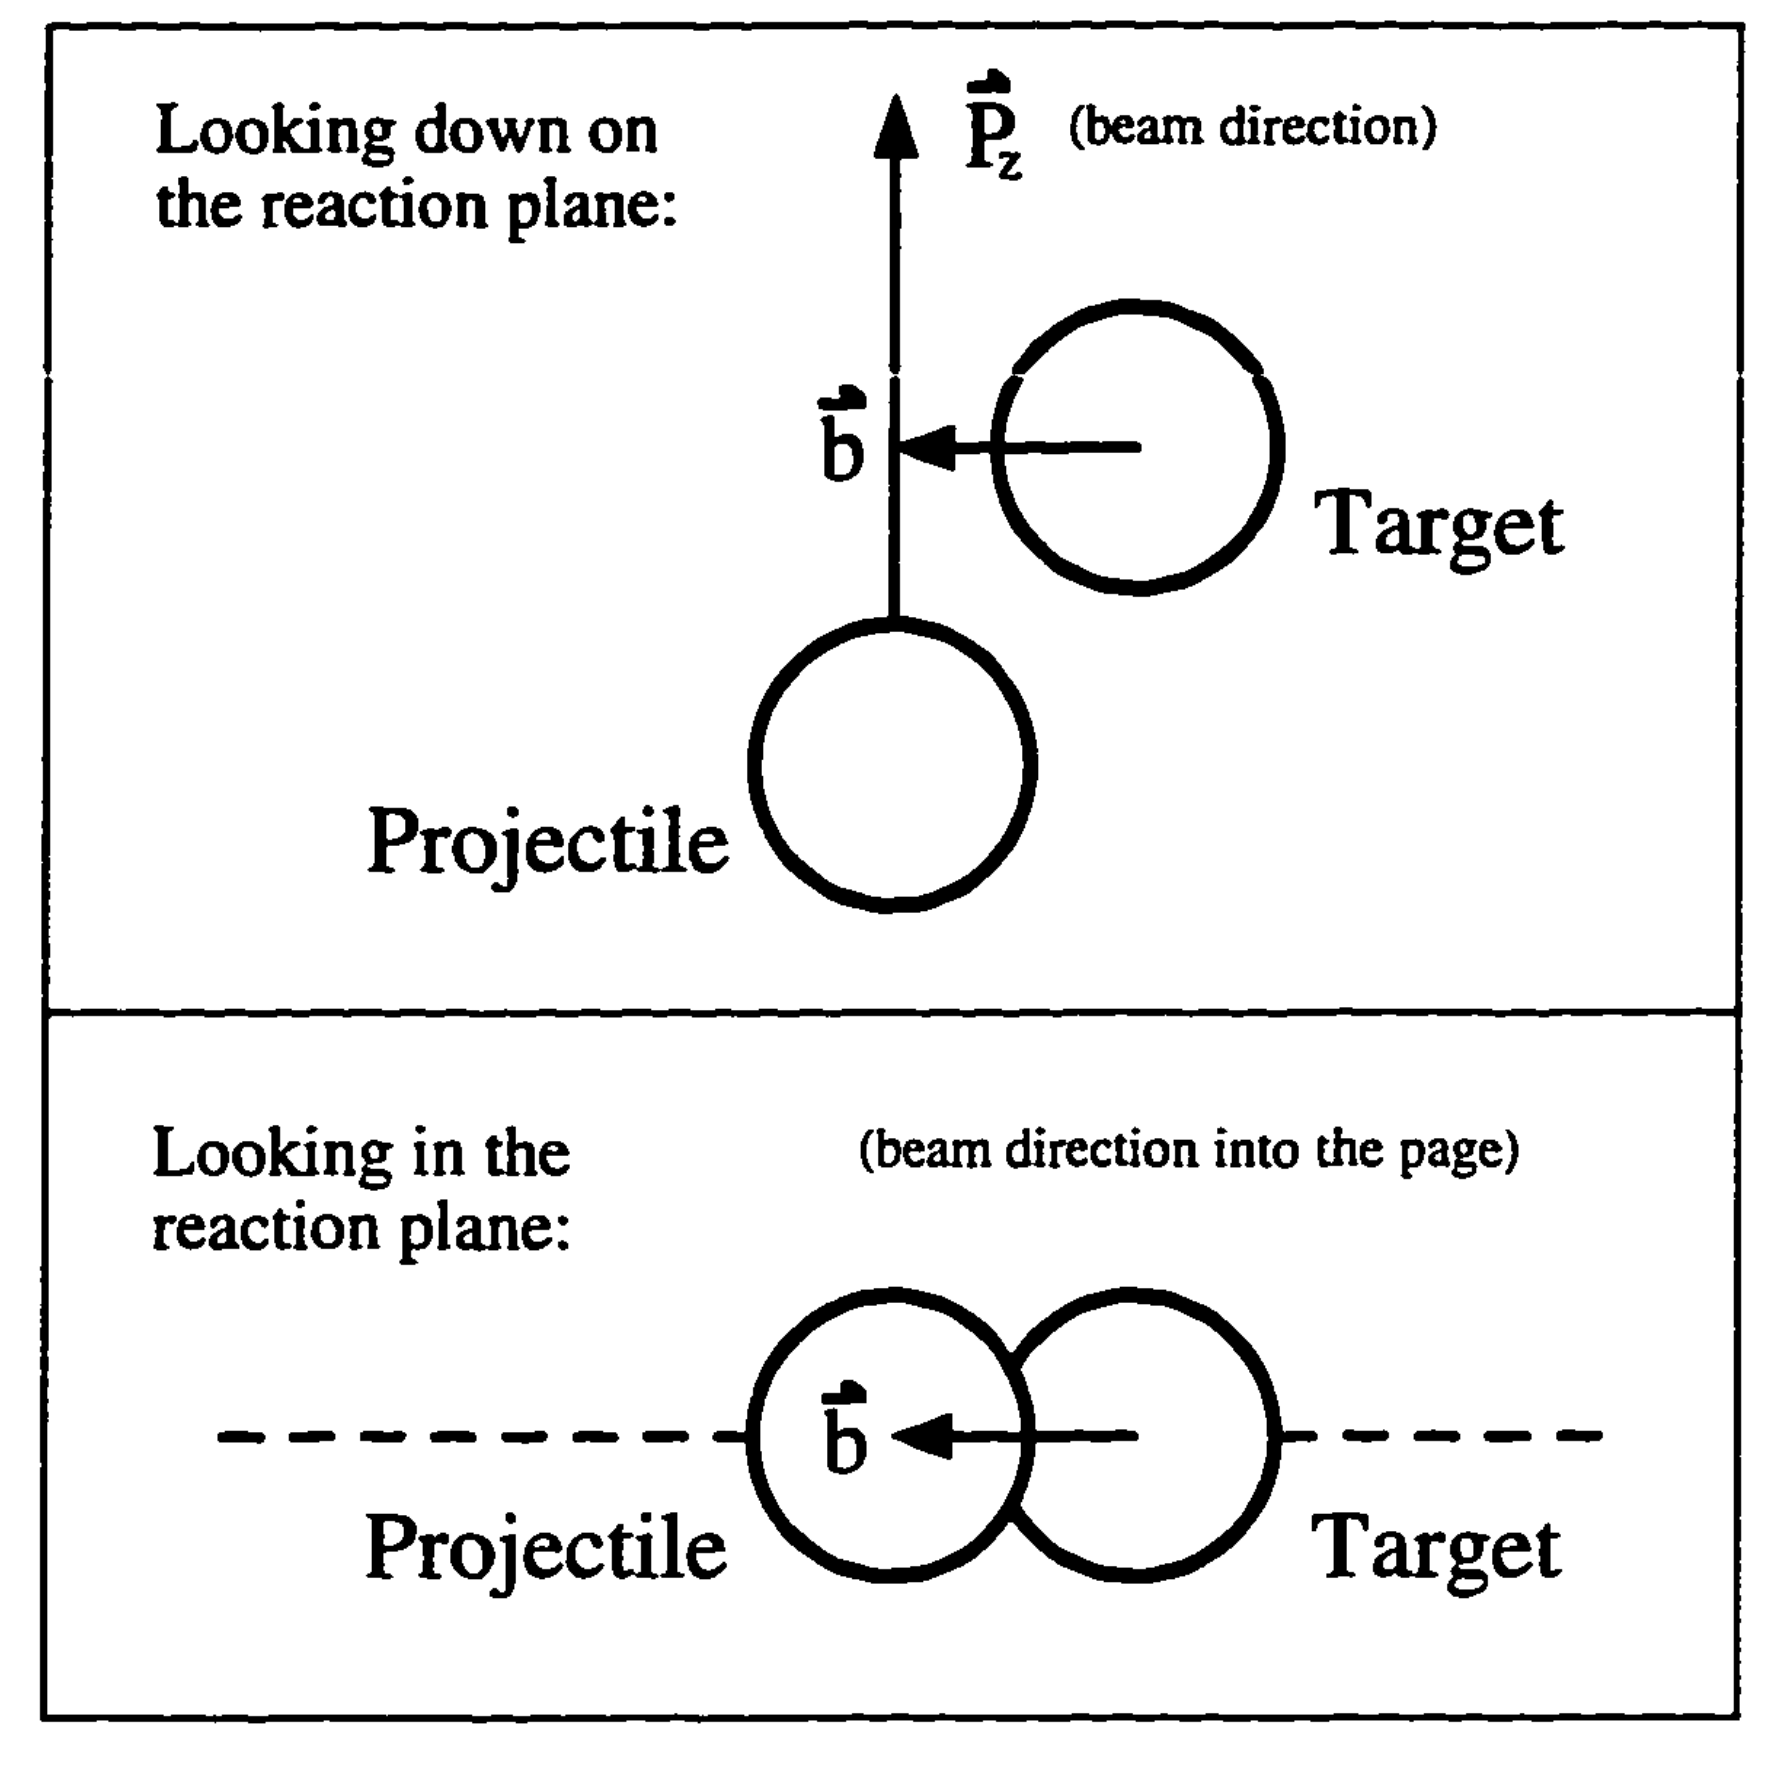
\includegraphics[width=\textwidth]{dad-thesis-figure}               
  One of the figures I helped my dad draw on a computer for his thesis, ``Collective flow in intermediate energy heavy-ion collisions,'' in 1996. Perhaps one day, I too will understand what it means.
\end{marginfigure}

\newthought{To my mother and father}, Dr. Robert and Myung-Hee Pak. My father, who was the first PhD in his own family, whom I remember happily marching down the aisles of the Breslin Center to the honks of Pomp and Circumstance for his doctorate in nuclear physics. Dad, you've been the role model for my life. Ever since I helped draw two figures for your thesis on the Macintosh you got me as a kid, proudly feeling like I had just put the torch on the Statue of Liberty, I've been wondering what it would be like to write one of my own. Well, have I got some bedtime reading material for you! And my mother, who kept me alive and kicking from a single cell all the way to whatever I am today, which if you think about it, is more remarkable than anything you will read in this dissertation. This never could have been written had it not been for my mother's ferocious dedication toward making a better life for me. Thanks, ma!

\newthought{To my thesis advisor}, Dr. Andrew Kasarskis, for taking me under his wing for the past four years. I am supremely lucky to have met somebody with the rare blend of patience, humor, genuine scientific curiosity, and mentorship skills that Andrew has and shares with others so freely. Andrew has taught me more than just science—he has taught me about leadership, entrepreneurship, integrity, life, and occassionally, wildlife. I look forward to pondering his lessons for the rest of my career. And to my fellow Kasarskis brother from the halls of Regis, the inimitable Dr. Joseph R. Scarpa, who blazed a trail for us both and kept me company as we jockeyed desks in Greenland. I am fortunate to be returning to medical school at his side.

\newthought{To the boys of 7G}, who are back in town, spread the word around. Kevin ``Carpet'' Hoffman, Michael ``The Stuffer'' Daniel, Zachary ``BJ'' Lorsch, Eddie ``Other Ted'' Contijoch, and Ranjan ``Gammie'' Upadhyay were my roommates as we began this strange and imprudent quest toward a dual degree. Then there's Andrew T. McKenzie, a late but profitable addition to the gang, who singlehandedly doubled our weirdness quotient and may just achieve his goal of a completely rational life strategy within the decade. And my entire entering class of 2012, who shall be rightfully remembered as ``the Titans.'' We have been through much together: retreats, pyramids, marathons, camping trips, uninhibited human flight, weddings, even a Tough Mudder—many of which could be considered a microcosm of certain aspects of the MSTP experience, but all of which I will always remember. You all kept me variously motivated, alive, and inspired throughout this ignoble quest, and I'll enjoy seeing you all crush it at science, medicine, and life.

\newthought{To the entire Sinai MSTP}, starting with the director from when I entered, Dr. Yasmin Hurd, and the many other leaders that have guided me since: Dr. Margaret Baron, Dr. Talia Swartz, Dr. Benjamin Chen, and Dr. Scott Friedman, to name a few. To the many other students in the program that gave me guidance and support, not least of all Dr. Benjamin Laitman, who was one of the first Sinai students I met, who steadfastly supported me through the challenges of leading Student Council, and whom I am honored to call my friend.

\newthought{To my colleagues in science}, who are also listed in acknowledgements within each chapter, but whom I must thank here not only for their collaborative efforts but also their friendship, mentorship, and personal support. From the Icahn Institute and Department for Genomics and Multiscale Biology: El-Ad David Amir, Oliver Attie, Ali Bashir, Harm van Bakel, Kieran Chacko, Brianne Ciferri, Gintaras Deikus, Gang Fang, Zeynep Gumus, Seunghee Kim-Schulze, Martha Lewis, David Nathanson, Leah C. Newman, Tim O'Donnell, Adeeb Rahman, Eric Schadt, Erick Scott, Robert Sebra, Mayte Suarez-Fariñas, Mitchell Sullivan, Maria Suprun, and Elizabeth Webster. From the Departments of Medicine and Pathology of the Mount Sinai Hospital: Judith Aberg, Camille Hamula, Jonathan Hand, Shirish Huprikar, Gopi Patel, Timothy Sullivan, and Fran Wallach. From the Department of Microbiology of the Icahn School of Medicine at Mount Sinai: Ana Fernandez-Sesma, Rebecca Hamlin, and Irene Ramos-Lopez, aka the Divas of Virology, who were so amazing to work with. To my colleagues from other institutions in the Dengue Human Immune Profiling Consortium, including Eva Harris and Daniela Michlmayr from UC Berkeley and Steven Wolinsky and Eun-Young Kim from Northwestern. There are likely many more scientists that quietly contributed their technical insight and effort to some aspect of the protocols, techniques, and datasets that eventually became a part of this dissertation, and for all of these unsung heroes whom I may never even meet, I want to express my sincere gratitude. 

\newthought{There are many other unsung heroes} in and around Mount Sinai whose support has been invaluable. Firstly, Courtney Manning, Gayle Schneiderman, and Rhaisili Rosario, who all did gangbusters work in keeping the MSTP running. Dr. Rainier P. Soriano, Dr. Yasmin Meah, Dr. David C. Thomas, Paul Lawrence, and Dr. David Muller gave me crucial guidance at certain points in the journey. I was lucky to have advice from Geoffrey Smith and Dan Seltzer on starting my business, The East Harlem Software Company, Inc. I have to thank the staff of Aron Hall, for maintaining such a nice home for all of us students. The guys at El Aguila on 103rd and Lex, whose tortas Cubanas fueled the improbable appearance of many words on these pages (which I recently learned is not an actual food in Cuba, but such is America). No acknowledgements could be complete without saluting Andy Efros, literally the nicest guy at Mount Sinai.

\newthought{I especially want to thank} Dr. Deena Altman for her dedicated leadership and evangelism of the Pathogen Surveillance Program, whose clinical insight and contributions made much of this dissertation possible before I even began, and who supported me from the first day I joined the group. As I go back into the hospital for clerkships and wonder what kind of doctor I want to be, I will be thinking often of Deena.

\newthought{To the members of my thesis advisory committee}: Dr. Adolfo García-Sastre, Dr. Jun Zhu, Dr. Joel Dudley, Dr. Jonathan Karr, and the chair Dr. James Iatridis, for providing focused guidance in developing this dissertation and meticulously supporting my development as a scientist. Special thanks to Dr. Bo Shopsin from the NYU School of Medicine, who graciously agreed to be an outside reviewer. To my undergraduate mentor, Dr. Frederick ``Fritz'' Roth, and members of his laboratory, who supported me throughout and after college, and first inspired me to pursue a doctorate in bioinformatics.

\newthought{Finally, I'd like to thank} Dr. Sonia Yen Jarrett, the only lady brave enough to put up with my shenanigans, who has kept me motivated throughout challenges I once thought impossible, and who always makes me laugh.

%%%%%%%%%%%%%%%%%%%%%%%%%%%%%%%%%%%%%%%%%%%%%%%%%%%%%%%%%%%%%%%%%%%%%%
% -*-latex-*-